\chapter{序論}
\section{研究背景}
深層学習は,現在多くの分野で利用されており,現代の科学技術において欠かせない技術の一つである.高性能な深層学習モデルを実現するためには,より大規模なデータセットの使用や,それに適したモデルのパラメータ設定が重要であるとされている.
従来,機械学習モデルの性能は,underfittingとoverfittingのトレードオフによって説明されてきた.訓練データが不足し,モデルのパラメータ数が少ない場合にはunderfittingが発生し,テストデータに対する性能が十分に向上しない.一方,訓練データに対してパラメータ数が過剰な場合にはoverfittingが生じ,テストデータに対する性能が低下する.このような現象は,一般にバイアス-バリアンスのトレードオフとして広く知られている\cite{Rajnarayan2017-ml}.
しかし,近年の研究では,モデルのパラメータ数が非常に大きくなると,一度はoverfittingによってテストデータに対する性能が低下するが,再び上昇する現象が観測された.この現象は,Belkinら\cite{Belkin2018-yx}によって発見され,「二重降下現象(double descent)」と名付けられた.さらに,Nakkiranらの研究では,DNNモデルにおいてパラメータ数の増加だけでなく,学習エポック数の増加によっても二重降下現象が生じることが確認されている\cite{Nakkiran2021-vf}.二重降下現象は,特に訓練データに対して,ラベルノイズを付与した場合の過学習が起きやすい場合に顕著に現れる.
こうした背景の中,\UTF{9AD9}橋ら\cite{DD_STB}はResNet18とCIFAR-10を用いて,二重降下現象と形状・テクスチャバイアスの関連性を示唆する研究を行った.この研究では,二重降下現象が発生する過程で,形状バイアスとテクスチャバイアスが逆転する現象が確認され,モデルの汎化性能が低下する段階において,これらのバイアスが影響していることが示された.

\section{研究目的}
この結果は,学習モデルが形状やテクスチャといった特徴を学習する過程に新たな洞察を与えたものの,色や数字といったよりシンプルな概念の学習過程については未だ明らかにされていない.そこで本研究では,異なる概念の獲得過程を明らかにするために,EMNIST Digitsデータセットを用い,色の概念を付与した数字データを対象として分類タスクを設定した.これにより,色クラスと数字クラスという2つの概念がどのように学習されるかを観測し,特にテスト誤り率に加えて,色のみの誤り率と数字のみの誤り率を同時に解析することで,複数の概念がどのように獲得されるのかを検証した.
深層学習モデルにおける概念獲得メカニズムの解明は,より効率的かつ解釈可能な機械学習モデルの開発に寄与すると考えられる.したがって,二重降下現象と概念獲得の関連を探ることで,CNNモデルにおける概念獲得過程の理解が深まり,より効果的なモデル構築への貢献が期待される.

\begin{figure}[t]
\centering
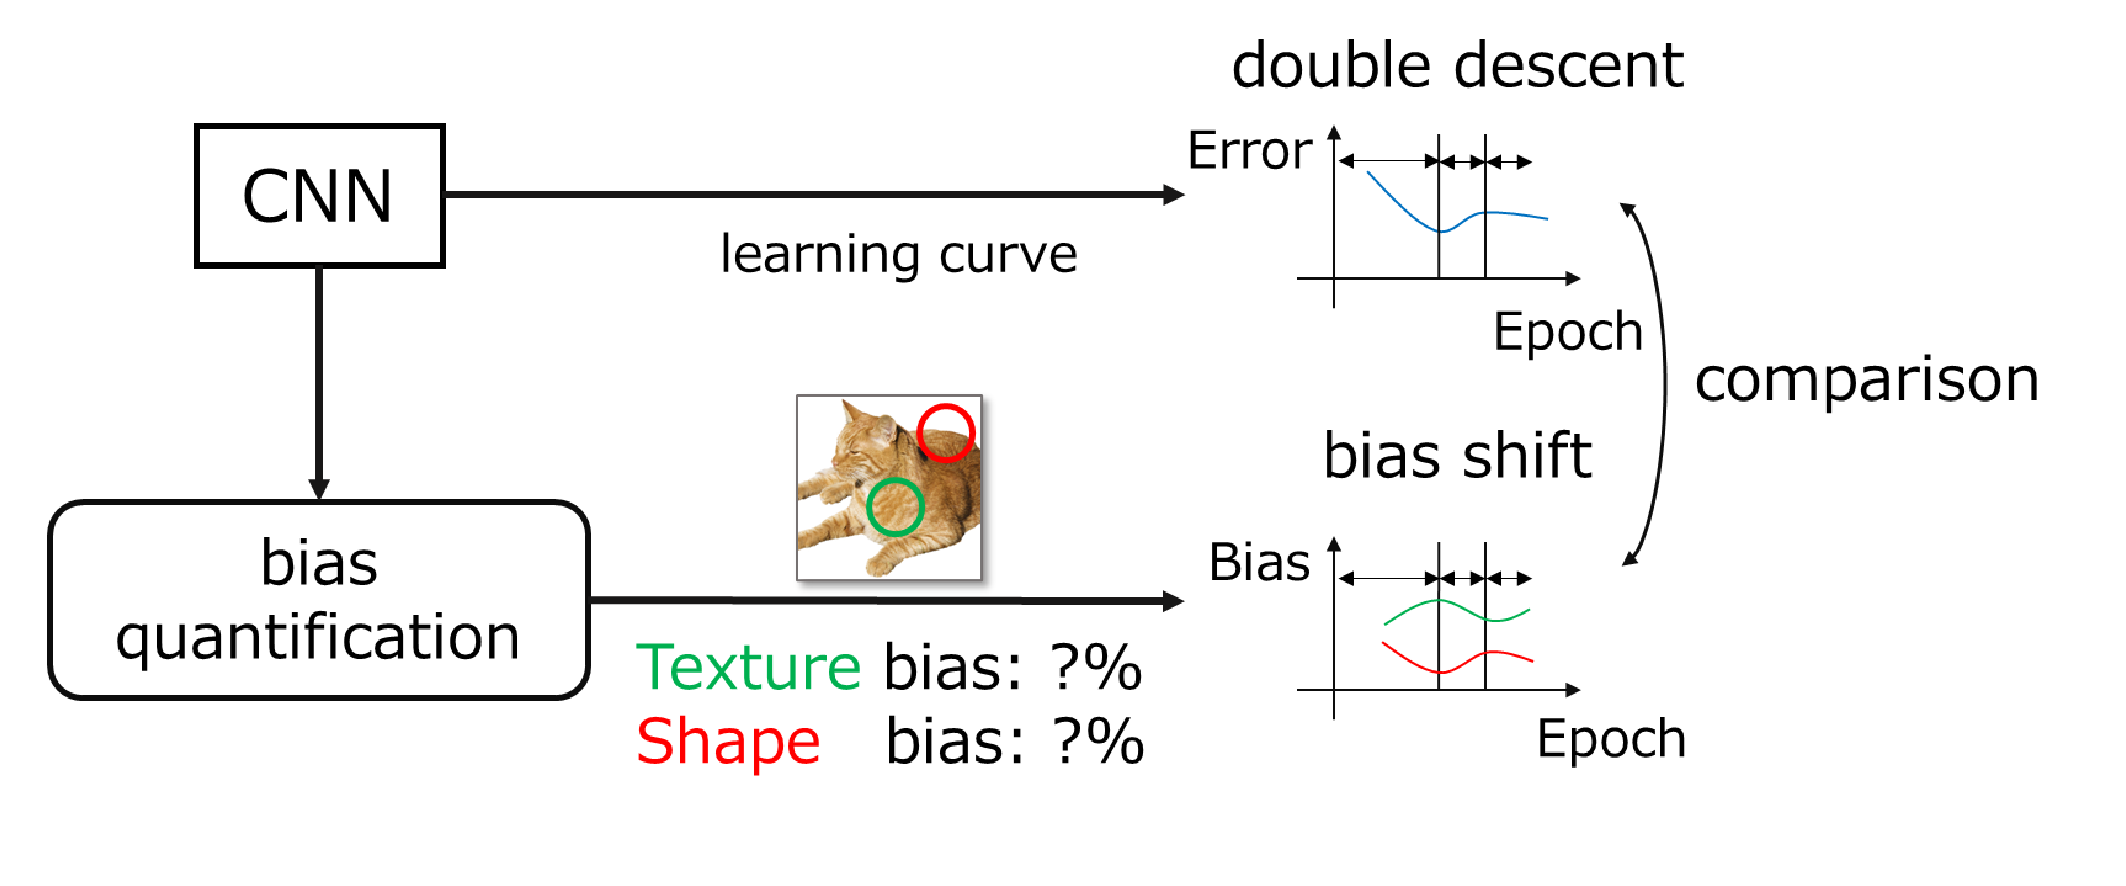
\includegraphics[width=1\columnwidth]{fig/fig1.pdf}
\vspace{-40pt}
\caption[ Flow of the analysis process comparing double descent with the learning process of image features.]{
% 本稿で紹介する解析プロセスの流れ。我々は畳み込みニューラルネットワーク(CNN)を採用し、二重降下条件下で多様な画像認識タスクを訓練した。形状/テクスチャのバイアスとテストエラーの時間的変化を監視し、形状やテクスチャを解釈するモデルの能力を評価すると同時に、それらの相関関係を探った。
%  Flow of the analysis process comparing double descent with the learning process of image features. We employed convolutional neural networks (CNNs) to train diverse image recognition tasks under double descent conditions. We monitored the temporal evolution of the shape/texture biases and test errors metrics assessing the capacity of the model to interpret shapes and textures while also exploring their correlation.
}
\label{fig:fig2}
\end{figure}

\section{論文構成}
第1章「序論」では昨今における深層学習の隆盛,深層学習にける既存理論と経験的観測との乖離,深層学習における性質といった背景,及びそれらを理解するための着想と本研究の目的を述べた.\par
第2章「先行研究」では,深層学習,二重降下現象,形状・テクスチャバイアスと二重降下現象の関係性について画像認識における深層学習モデルの理解に関して述べる.\par
第3章「深層学習における二重降下現象と概念獲得」では,本研究において不可欠な深層学習における学習過程について,実験設定と結果を述べる.\par
% 第4章「自然画像が持つ特徴に着目した分析」では,画像固有の特徴(形状・テクスチャ)と二重降下現象の関係を掘り下げるために必要な実験設定について述べる.\par
% 第5章「実験」では,第4章に基づいて行った検証結果,各種パラメータが与える実験結果への影響について検証する.\par
% 第6章「追加実験」では,モデルが持つ層ごとの学習過程に着目し,検証する.\par
% 第7章「考察」では,実験結果についての考察を行う.\par
% 第8章「結論」では,本研究を総括する.\par
% % 第9章「今後の展望」では,本研究で得られた知見から今後の方向性を示す.\par
\newpage